%%%%%%%%%%%%%%%%%%%%%%%%%%%%%%%%%%%%%%%%%%%%%%%%%%%%%%%%%%%%%%%%%%%%%
% PREAMBLE
%%%%%%%%%%%%%%%%%%%%%%%%%%%%%%%%%%%%%%%%%%%%%%%%%%%%%%%%%%%%%%%%%%%%%
%
% The following two commands will generate a PDF that follows all the 
% requirements for submission and peer review.  Uncomment these commands 
% to generate this output (and comment out the two lines below.)
%
% DOUBLE SPACE VERSION FOR SUBMISSION TO THE AMS
\documentclass[12pt]{article}
\usepackage{ametsoc}
\usepackage[pagewise]{lineno}
\linenumbers
%
% The following two commands will generate a single space, double column 
% paper that closely matches an AMS journal page.  Uncomment these commands 
% to generate this output (and comment out the two lines above. FOR AUTHOR 
% USE ONLY. PAPERS SUBMITTED IN THIS FORMAT WILL BE RETURNED
% TO THE AUTHOR for submission with the correct formatting.
%
% TWO COLUMN JOURNAL PAGE LAYOUT FOR AUTHOR USE ONLY
%%%%\documentclass[10pt]{article}
%%%%\usepackage{ametsoc2col}
%
%%%%%%%%%%%%%%%%%%%%%%%%%%%%%%%%%%%%%%%%%%%%%%%%%%%%%%%%%%%%%%%%%%%%%
% ABSTRACT
%
% Enter your Abstract here
%%%%%%%%%%%%%%%%%%%%%%%%%%%%%%%%%%%%%%%%%%%%%%%%%%%%%%%%%%%%%%%%%%%%%
\newcommand{\myabstract}{
Direct measurements of rates of entrainment into and detrainment from 
cumulus cloud cores obtained from LES model cloud fields produce values 
twice as large as those produced from tracer budget calculations.  This 
difference can be explained by two effects: the presence of a shell of 
moist air around the cloud cores and drier air at the edge of the cloud 
core, and the tendency for the mean tracer value of the entrained fluid 
to be greater than the mean tracer value of the cloud shell. Preferential 
entrainment of shell air that is moving upward faster than the mean shell 
creates strong vertical momentum fluxes into the cumulus cloud core, 
making the assumption that cumulus clouds entrain fluid with zero 
vertical momentum incorrect.  Variability in the properties of the moist 
cloud shell has strong impacts on entrainment values inferred from tracer 
budget calculations.  These results indicate the dynamics of the cloud 
shell should be included in parametrization of cumulus clouds used in 
general circulation models.
}
%
\begin{document}
%
%%%%%%%%%%%%%%%%%%%%%%%%%%%%%%%%%%%%%%%%%%%%%%%%%%%%%%%%%%%%%%%%%%%%%
% TITLE
%
% Enter your TITLE here
%%%%%%%%%%%%%%%%%%%%%%%%%%%%%%%%%%%%%%%%%%%%%%%%%%%%%%%%%%%%%%%%%%%%%
\title{\textbf{\large{The influence of the cloud shell on tracer budget 
measurements of LES cloud entrainment}}}
%
% Author names, with corresponding author information. 
% [Update and move the \thanks{...} block as appropriate.]
%
\author{\textsc{Jordan T Dawe}
		\thanks{\textit{Corresponding author address:} 
				Jordan T Dawe, Department of Earth and Ocean Sciences, 
                University of British Columbia, 6339 Stores Road,
                Vancouver, BC, V6T 1Z4, Canada.
		\newline{E-mail: jdawe@eos.ubc.ca}}\quad\textsc{and Philip H Austin}\\
\textit{\footnotesize{Department of Earth and Ocean Sciences, University of 
                      British Columbia, Vancouver, BC, Canada.}}
}
%
% Formatting done here...Authors should skip over this.  See above for abstract.
\ifthenelse{\boolean{dc}}
{
\twocolumn[
\begin{@twocolumnfalse}
\amstitle

% Start Abstract (Enter your Abstract above.  Do not enter any text here)
\begin{center}
\begin{minipage}{13.0cm}
\begin{abstract}
	\myabstract
	\newline
	\begin{center}
		\rule{38mm}{0.2mm}
	\end{center}
\end{abstract}
\end{minipage}
\end{center}
\end{@twocolumnfalse}
]
}
{
\amstitle
\begin{abstract}
\myabstract
\end{abstract}
}
%%%%%%%%%%%%%%%%%%%%%%%%%%%%%%%%%%%%%%%%%%%%%%%%%%%%%%%%%%%%%%%%%%%%%
% MAIN BODY OF PAPER
%%%%%%%%%%%%%%%%%%%%%%%%%%%%%%%%%%%%%%%%%%%%%%%%%%%%%%%%%%%%%%%%%%%%%
\section{Introduction}

The rate at which air is entrained into and detrained from cumulus clouds 
affects cloud properties, cloud top height, and vertical transports of heat 
and moisture.  Proper simulation of cumulus sub-grid scale fluxes in General 
Circulation Models (GCM) depends on the accurate parametrization of 
entrainment of environmental tracer properties into the clouds and detrainment 
of cloud properties into the environment 
\citep{Bechtold2008, De_Rooy2010}.  

Entrainment and Detrainment may be defined mathematically as
\begin{subequations}
 \label{eq:ED_theoretical}
\begin{equation}
E = -\frac{1}{A}\oint_{\mathbf{\hat{n}}\cdot(\mathbf{u} - \mathbf{u_i}) < 0}
\rho\mathbf{\hat{n}}\cdot(\mathbf{u}-\mathbf{u_i})dl
\end{equation}
\begin{equation}
D = \frac{1}{A}\oint_{\mathbf{\hat{n}}\cdot(\mathbf{u} - \mathbf{u_i}) > 0}
\rho\mathbf{\hat{n}}\cdot(\mathbf{u}-\mathbf{u_i})dl
\end{equation}
\end{subequations}
where $E$ and $D$ are the entrainment and detrainment rates in kg m$^{-3}$ 
s$^{-1}$, $\rho$ is the density of air in kg m$^{-3}$ s$^{-1}$, $\mathbf{u}$ is 
the velocity of the air in m s$^{-1}$, $\mathbf{u_i}$ is the velocity of the 
cloud surface in m s$^{-1}$, A is the area of the cloud in m$^2$, 
$\mathbf{\hat{n}}$ is a unit vector directed out the cloud surface, and the 
path integral is taken around the cloud surface at a constant vertical level 
\citep{Siebesma1998}.  Entrainment and detrainment are thus caused by 
differences between the motion of the cloud surface and the motion of the air.  
This includes not just mixing processes, but also adiabatic processes such as 
condensation of fluid at cloud base.  Many parameterizations use cloud core as 
the region over which to consider entrainment and detrainment, defined as
regions having condensed liquid water, positive buoyancy, and upward vertical
velocity.  In this case, the motion of the cloud core surface is simply 
substituted for the motion of the cloud surface in equations 
(\ref{eq:ED_theoretical}).

Entrainment and detrainment rates impact GCM parameterizations in several ways.
First, profiles of cloud vertical mass flux are usually calculated from 
parametrized entrainment values using the continuity equation for a 
simple entraining plume to represent an ensemble of cumulus clouds:
\begin{equation}
   \label{eq:continuity}
   \rho \frac{\partial a}{\partial t} 
   + \frac{\partial M_{core}}{\partial z} = E - D.
\end{equation}
Here $a$ is the fractional cloud core area  and $M_{core}$ is vertical cloud 
core mass flux (kg m$^{-2}$ s$^{-1}$). The level where the mass flux profile 
goes to zero then defines the location of the cloud ensemble top.  This mass 
flux profile is combined with the entrainment rate of environmental air into 
the cloud and the detrainment rate of cloud air into the environment to 
generate vertical profiles of cloud water vapor, condensate, and 
temperature, and these profiles are then used to calculate the moistening 
of the environment by detrainment of cloud fluid 
\citep{Tiedtke1989, Kain1990}.  Precipitation rates are also generated from the
mass flux and tracer profiles produced from the entrainment and detrainment
profiles.  This wide variety of effects make entrainment rate one of the 
strongest controls on the climate sensitivity of GCMs 
\citep{Stainforth2005, Rougier2009}.

Large Eddy Simulation (LES) is the primary tool used to study cloud entrainment.  
LES mass entrainment and detrainment rates are typically obtained using budgets 
of conserved tracer variables to infer the amount of fluid exchange between the 
cloud ensemble and the surrounding air.  \cite{Siebesma1995} derive the 
following equations for entrainment and detrainment of mass from the 
ensemble of cloud core plumes:
\begin{subequations}
  \label{eq:siebesmaED}
\begin{equation}
  \label{eq:siebesma_entrainment}
    E_{\phi}(\phi_{core} - \phi_{env}) = 
        - M_{core} \frac{\partial \phi_{core}}{\partial z}
        - \frac{\partial \rho a \overline{w' \phi'}^{core}}{\partial z}
        - \rho a \frac{\partial \phi_{core}}{\partial t}
        + a \rho \left(\frac{\partial \bar{\phi}}{\partial t}\right)_{forcing}
\end{equation}
and
\begin{equation}
  \label{eq:siebesma_detrainment}
    D_{\phi}(\phi_{core} - \phi_{env}) = 
        - M_{core} \frac{\partial \phi_{env}}{\partial z}
        + \frac{\partial \rho (1 - a) \overline{w' \phi'}^{env}}{\partial z}
        + \rho (1-a) \frac{\partial \phi_{env}}{\partial t}
     - \rho (1-a) \left(\frac{\partial \bar{\phi}}{\partial t}\right)_{forcing}
\end{equation}
\end{subequations}
Where $\phi$ (with units denoted by $[\phi]$) represents any conserved tracer, 
such as the total specific humidity $q_t$ (kg water kg$^{-1}$ moist air) or the 
liquid-water moist static energy $h$ (J kg$^{-1}$); $w$ is vertical velocity 
(m s$^{-1}$); $env$ and $core$ sub-and super-scripts denote horizontally
averaged values conditionally sampled in the cloud environment and
core; $forcing$ refers to tracer sources and sinks, such as radiation
or large-scale subsidence, not included in the other terms; primed values
represent anomalies relative to the horizontal mean; overbars represent 
horizontal averaging; and $E_{\phi}(z)$ and $D_{\phi}(z)$ are the total 
mass entrainment into and detrainment from the cloud core inferred from 
the tracer budget, in kg s$^{-1}$ m$^{-3}$.  Under this budget formulation,
$E_{\phi}(z)$ and $D_{\phi}(z)$ consist of all horizontal mass exchanges
between clouds and their environment, including advective processes, 
diffusive processes, and thermodynamic phase changes. We shall refer to 
values calculated by this method as ``tracer budget" entrainment and 
detrainment. For convenience, the various tracer and entrainment/detrainment 
rate subscripts used below are summarized in the Appendix.

Alternatively, entrainment and detrainment of mass can be calculated directly
from the LES velocity and tracer fields.  \cite{Romps2010} recently presented a 
technique to measure local (grid scale) mass entrainment $e(x,y,z)$ and
detrainment $d(x,y,z)$.  His equation (2) is:
\begin{equation}
  \label{eq:romps_e_minus_d}
  e - d = \frac{\partial}{\partial t}(\mathcal{A}\rho) 
        + \nabla \cdot (\rho \mathbf{u} \mathcal{A}) 
\end{equation}
Here $\mathcal{A}$ is the ``activity'' of the fluid, where
$\mathcal{A}$ is one at cloud core points and zero otherwise.  The values of
$e - d$ are averaged over the time that a grid cell experiences mass
fluxes between an active and an inactive point, then positive $e-d$
values are considered to be purely $e$, and negative values, $d$.  
Summing these point measurements horizontally gives 
$E_d(z)$ and $D_d(z)$, the total mass entrained into and detrained from the
cloud core field in kg s$^{-1}$ m$^{-3}$, where the $d$ subscript indicates 
these quantities were calculated directly from the model velocity and tracer
fields.  We shall refer to entrainment and detrainment values
calculated by this method as ``direct" entrainment and detrainment.

Romps found that such direct calculation of the entrainment and
detrainment mass fluxes produced values roughly twice as large as
tracer budget calculations.  Romps attributed this difference to the 
tracer budget calculation assumption that fluid exchanged between clouds 
and environment has the mean properties of the cloud or environment at 
that level, respectively.  Studies of the dense, descending shell of 
moist air that forms around trade-wind cumulus clouds 
\citep{Jonas1990, Rodts2003, Heus2008, Jonker2008, Heus2009, Wang2010} 
suggest that the cloud shell properties are quite different than the core 
or environment properties, bolstering Romps' hypothesis.  Since fluid 
exchanges between clouds and environment must pass through this shell, it 
is likely that it plays an important role in entrainment and detrainment
dynamics.

Below we examine the sources of the discrepancy in entrainment and
detrainment values calculated via tracer budgets and directly
using (\ref{eq:romps_e_minus_d}).  We show that the discrepancy is explained by 
two effects: the presence of the shell of moist air around the cloud cores
and drier air at the edge of the cloud core, and preferential entrainment of 
shell air with higher average humidity and upward velocity than the mean shell 
properties which enhances tracer fluxes between the clouds and the environment.
We derive a relation to transform the direct mass entrainment and detrainment 
fluxes into tracer budget values suitable for use in one-dimensional simple 
entraining plume cloud parameterizations, and then use these transformed fluxes 
to evaluate the impact of the shell on tracer budget entrainment and 
detrainment rates of specific humidity and vertical velocity.  Finally, we
examine the dynamics that drives the preferential entrainment of air with 
higher than average specific humidity and vertical velocity.

%===================================================

\section{Model description}

All LES calculations in this paper were made using the System for Atmospheric 
Modeling \citep[SAM;][]{Khairoutdinov2003}.  Two model runs were performed, 
configured as standard Global Energy and Water Cycle Experiment (GEWEX) 
Cloud System Studies \citep[GCSS;][]{Randall2003} experiments: a Barbados 
Oceanographic and Meteorological Experiment \citep[BOMEX;][]{Siebesma2003} run,
and an Atmospheric Radiation Measurement Study \citep[ARM;][]{Brown2002} run. 
The BOMEX run was performed on a 6.4 km x 6.4 km horizontal x 3.2 km vertical 
domain with 25 meter grid size in all directions for 6 hours, and the first 
three hours of simulation were discarded. The ARM run was performed on a 
7.68 km x 7.68 km x 4.5 km domain with 30 meter grid size.  Precipitation was 
disabled in both runs.

We have implemented the direct entrainment calculation scheme of 
\cite{Romps2010} in SAM, allowing us to calculate the mass of air 
entrained into and detrained from cloud core directly from model $\rho$, 
$\mathbf{u}$, and $\mathcal{A}$.  \citet[eq. 4]{Romps2010} also 
presents a method for calculating local entrainment and detrainment rates 
for any model variable in the same framework as (\ref{eq:romps_e_minus_d}),
but neglects forcing terms.  These terms are significant for quantities 
like vertical momentum, so we modify Romps' equation to include their 
effects:
\begin{equation}
  \label{eq:romps_ephi_minus_dphi}
  e\phi - d\phi = \frac{\partial}{\partial t}(\phi \mathcal{A} \rho) 
                + \nabla \cdot (\phi \rho \mathbf{u} \mathcal{A})
                - \rho \mathcal{A}S_\phi.
\end{equation}
where $S_\phi$ is any non-advective and non-diffusive source or sink term for 
$\phi$, such as precipitation for $q_t$ or pressure gradient for $w$, in units 
of $[\phi]$ s$^{-1}$.  Diffusion is excluded from $S_\phi$ as it is 
part of the entrainment/detrainment process, and so is included in the 
$e\phi - d\phi$ term of the equation.  The inclusion of these source/sink 
terms allows us to expand the definition of $\phi$ to include non-conserved 
fluid properties.

As with equation (\ref{eq:romps_e_minus_d}), the local $(e\phi)(x,y,z)$
and $(d\phi)(x,y,z)$ must be horizontally summed to give the total entrainment 
into or detrainment out of the cloud ensemble for any fluid property, but
since $\phi$ can be negative for properties like vertical velocity, it is 
possible for entrainment to reduce and for detrainment to increase the 
various properties of the cloud core.  To accommodate this effect, if the 
average value of $\phi$ is positive over the time that a grid cell experiences 
mass fluxes between an active and an inactive grid cell, then positive 
$e\phi-d\phi$ values are considered to be purely $e\phi$, and negative values, 
$d\phi$.  However, if the average of $\phi$ is negative, then positive 
$e\phi-d\phi$ values are considered to be purely $(d\phi)(x,y,z)$, and negative 
values, $(e\phi)(x,y,z)$.

The obvious way to calculate the average value of $\phi$ is to perform a 
flux-weighted calculation, so that $\phi = (e\phi - d\phi)/(e - d)$.  
However, doing so for positive definite quantities, such as total specific 
water $q_t$, sometimes results in negative $\phi$.  To see the reason 
for this, consider a situation where $(e - d)$ integrated over the period 
that a grid cell is active is found to be slightly bigger than zero for 
a grid cell.  The Romps algorithm would assign $e$ to a small value and 
$d$ to be zero, but this is only one of many equally valid choices; as 
long as $e \approx d$, the net flux measured by the algorithm would be 
satisfied.  At the same time, $(e q)_d - (d q)_d$ 
($(e \phi)_d - (d \phi)_d$) using $q_t$ for $\phi$) is found to be 
negative, presumably due to $e$ and $d$ having similar magnitudes while 
the detraining air has higher humidity than the entraining air.  In this 
case, $((e q)_d - (d q)_d)/(e-d)$ will be negative, even though $q_t$ is 
always positive.  To avoid this problem, we calculate $\phi$ as a simple 
time average for the purpose of determining if $e\phi-d\phi$ is 
assigned to $e\phi$ or to $d\phi$.  Horizontal summation of $(e\phi)$ 
and $(d\phi)$ then gives $(E\phi)_d(z)$ and $(D\phi)_d(z)$, the total 
entrainment and detrainment of a property for the cloud ensemble in 
units of $[\phi]$ kg s$^{-1}$ m$^{-3}$ calculated directly from the 
model velocity and property fields.

%===================================================

\section{Relationship Between Direct and Tracer Budget Entrainment}

\cite{Romps2010} established that the direct estimate of mass entrainment 
and detrainment yields values roughly twice the size of those calculated 
via conserved tracer budgets.  Furthermore, examination of the ratios of 
the mass entrainment and detrainment calculated via a total specific 
water budget ($E_q$, $D_q$) to the directly calculated values 
($E_d$, $D_d$) over the diurnal cycle of an ARM LES reveals significant 
changes over the course of the day 
(Fig.~\ref{fig:entrainment_ratio_variability}).  Thus, the direct and 
tracer budget measurements of $E$ and $D$ are not only significantly
different, but have differing dynamics, which may need to be be accounted 
for in large-scale parameterizations of cloud entrainment and detrainment.  
In this section we examine the sources of disagreement between direct and 
tracer budget estimates of mass entrainment into and detrainment from the 
cloud core.

%---------------------------------------------------

\subsection{$E$ and $D$ Cloud Shell Correction}

Romps attributed the differences between ($E_{\phi}$, $D_{\phi}$)
and ($E_d$, $D_d$) to the assumption made by \cite{Siebesma1995} that
fluid being entrained or detrained has the properties of the mean
environment or cloud core, respectively.  If we examine the horizontal 
mean specific humidity of the fluid at the ``cloud core edge" (cloud 
core model grid cells that are nearest-neighbor adjacent to non-core 
cells), which presumably is the fluid being detrained, we see it is 
indeed drier than the mean core (Fig. \ref{fig:Shell_correction}a).  
Similarly, the fluid available for entrainment in the ``cloud core shell" 
(non-core model grid cells that are nearest-neighbor adjacent to core 
cells) is moister than the mean environment.

Budget equations that explicitly distinguish between the mean cloud 
core and environment properties and the properties of the entraining 
and detraining fluid allow us to transform ($E_d, D_d$) values into 
equivalent tracer budget values, and back again.  We start our derivation
with the observation that both the tracer budget and direct values of 
$E$ and $D$ are consistent with the continuity equation (equations 
(\ref{eq:continuity}) and (\ref{eq:romps_e_minus_d})).  This implies  
\begin{equation}
  E_{\phi} - D_{\phi} = E_d - D_d.
\end{equation}
Similarly, the entrainment and detrainment rates of fluid properties 
must be consistent with the total property budget, giving us
\begin{equation}
  E_{\phi} \phi_{env} - D_{\phi} \phi_{core} = E_d \phi_E - D_d \phi_D,
\end{equation}
where $\phi_E$ and $\phi_D$ represent the $\phi$ of the fluid being 
entrained or detrained, respectively. Combining these equations and 
solving for $E_{\phi}$ and $D_{\phi}$ in turn results in:
\begin{subequations}
  \label{eq:correctedED}
\begin{equation}
  \label{eq:corrected_entrainment}
    E_{\phi,T} = E_d 
             - \left[E_d\frac{(\phi_E - \phi_{env})}
                             {(\phi_{core} - \phi_{env})}
                   + D_d\frac{(\phi_{core} - \phi_D)}
                             {(\phi_{core} - \phi_{env})}\right]
\end{equation}
\begin{equation}
  \label{eq:corrected_detrainment}
    D_{\phi,T} = D_d
             - \left[E_d\frac{(\phi_E - \phi_{env})}
                             {(\phi_{core} - \phi_{env})}
                   + D_d\frac{(\phi_{core} - \phi_D)}
                             {(\phi_{core} - \phi_{env})}\right].
\end{equation}
\end{subequations}
Here the $T$ subscript indicates these $E_{\phi}$ and $D_{\phi}$ 
tracer budget values have been calculated by transformation of direct 
values, not via equations (\ref{eq:siebesmaED}).  The bracketed terms 
represent the bias introduced by assuming that entrained/detrained air 
has the properties of the mean environment and core.  Thus, to convert 
from ($E_d$,$D_d$) to ($E_{\phi,T}$, $D_{\phi,T}$), both $E_d$ and $D_d$ 
must be reduced by $E_d A + D_d B$, where 
$A = (\phi_E - \phi_{env})/(\phi_{core} - \phi_{env})$ and 
$B = (\phi_{core} - \phi_D)/(\phi_{core} - \phi_{env})$.  

Note that rearrangement of $A$ gives 
$\phi_E = A \phi_{core} + (1-A)\phi_{env}$, meaning that $A$ can be 
thought of as the fraction of mean core air in a mixture of mean 
core and mean environment air needed to produce the properties of the 
entrained fluid.  Similarly, $\phi_D = B \phi_{env} + (1-B)\phi_{core}$ 
and $B$ can be thought of as the fraction of mean environment air in a 
mixture of mean core and mean environment air needed to produce the 
properties of the detrained fluid.  Since the fluid being entrained or 
detrained does not necessarily originate at the level it is entrained 
or detrained at, we cannot assume that a fraction $A$ of the entrained 
air is modified core air.  Nevertheless, $A$ and $B$ are likely related 
to the recirculation of entrained and detrained air.

Alternatively, we can solve for $E_d$ and $D_d$, arriving at
\begin{subequations}
\begin{equation}
  \label{eq:corrected_entrainment2}
    E_{d,T} = E_{\phi}
        + \left[E_{\phi}\frac{(\phi_E - \phi_{env})}
                               {(\phi_D - \phi_E)} 
              + D_{\phi}\frac{(\phi_{core} - \phi_D)}
                               {(\phi_D - \phi_E)}\right].
\end{equation}
\begin{equation}
  \label{eq:corrected_detrainment2}
    D_{d,T} = D_{\phi} 
        + \left[E_{\phi}\frac{(\phi_E - \phi_{env})}
                               {(\phi_D - \phi_E)}
              + D_{\phi}\frac{(\phi_{core} - \phi_D)}
                               {(\phi_D - \phi_E)}\right].
\end{equation}
\end{subequations}
Again, the $T$ subscript indicates these $E_d$ and $D_d$ values have 
been calculated by transformation of $E_{\phi}$ and $D_{\phi}$, not 
via equation (\ref{eq:romps_e_minus_d}).  In this case, to convert from 
($E_{\phi}$, $D_{\phi}$) to ($E_{d,T}$, $D_{d,T}$), both $E_{\phi}$ and 
$D_{\phi}$ must be increased by $E_{\phi} a + D_{\phi} b$, where 
$a = (\phi_E - \phi_{env})/(\phi_D - \phi_E)$ and 
$b = (\phi_{core} -\phi_D)/(\phi_D - \phi_E)$.

We now have relationships allowing us to transform the unbiased
$E_d$ and $D_d$ values into biased tracer budget
$E_{\phi}$ and $D_{\phi}$ values, which are better suited for
simple entraining plume parametrization of cloud fields.
Comparison of $E_q$ and $D_q$ ($E_{\phi}$ and $D_{\phi}$ inferred
using total specific moisture $q_t$ as the tracer) with $E_d$ and $D_d$
shows the direct entrainment and detrainment magnitudes are significantly larger 
than the tracer budget values (Figure \ref{fig:Shell_correction}b 
and \ref{fig:Shell_correction}c, grey and dotted lines).  
Using (\ref{eq:correctedED}) to calculate $E_{q,T}$ and $D_{q,T}$ with
$q_E = q_{edge}$, the horizontal mean humidity in the cloud edge, and 
$q_D = q_{shell}$, the horizontal mean humidity in the cloud shell, 
results in values quite close to the tracer budget values above the 
middle of the cloud layer. The transformation also duplicates the 
negative detrainment values near cloud base that are typically produced 
by tracer calculations.

%-------------------------------------------------------------------------

\subsection{Preferential Entrainment of Moist, Ascending Air}

Relative to the tracer budget values, the $E_{q,T}$ and 
$D_{q,T}$ values calculated using $q_E = q_{edge}$ and $q_D = q_{shell}$ 
are still too large near cloud base. We can explain this difference as 
being the result of the mean fluid property values of the entrained and 
detrained air being different than the mean value of the shell and edge 
air, respectively.  Using the mean shell and edge values of properties to 
transform the direct entrainment and detrainment assumes that any 
fluid parcel in the shell or edge is equally likely to be entrained or 
detrained.  In reality, mixing relatively dry air into the cloud core is 
more likely to cause evaporation, which will drive detrainment, while 
mixing relatively moist air into the cloud core is more likely to 
produce a saturated fluid mixture, resulting in entrainment.  This 
suggests that the moistest shell parcels are more likely to undergo 
entrainment than the average shell parcel, and the driest edge parcels 
are more likely to detrain than the average edge parcel.

We can directly calculate the effective fluid property values at which 
entrainment occurs by taking the total fluid property entrainment 
$(E\phi)_d$ (calculated via equation (\ref{eq:romps_ephi_minus_dphi}))
and dividing it by the total mass entrainment $E_d$ so that 
$\phi_{entrain} = (E\phi)_d / E_d$.  Similarly, the effective property 
values of the detraining air can be found from  
$\phi_{detrain} = (D\phi)_d / D_d$.  Examination of these values from
the BOMEX simulation using $q_t$ for $\phi$ shows $q_{entrain}$ is 
moister than $q_{shell}$ (Figure \ref{fig:Reynolds_correction}a), 
indicating entrainment occurs preferentially at the moistest parts 
of the shell.  Conversely, there is little difference between between 
$q_{detrain}$ and $q_{edge}$, indicating the detrained parcels tend to 
have the mean moisture of the cloud core edge.  Using $q_{entrain}$ and 
$q_{detrain}$ to transform $E_d$ and $D_d$ reduces the large entrainment 
and detrainment values near cloud base found using the mean shell and 
edge properties (solid black line, Fig.~\ref{fig:Reynolds_correction}b 
and \ref{fig:Reynolds_correction}c), bringing $E_{q,T}$ and $D_{q,T}$ 
into agreement with $E_q$ and $D_q$.

%==========================================================================

\section{$E_q$, $E_h$ and $E_w$ Differences}

Equations (\ref{eq:corrected_entrainment}) or 
(\ref{eq:corrected_detrainment}) imply that the tracer budget method will 
measure different entrainment and detrainment values for fluid properties 
with differing values of 
$A = (\phi_E - \phi_{env})/(\phi_{core} - \phi_{env})$ and
$B = (\phi_{core} - \phi_D)/(\phi_{core} - \phi_{env})$.  With this in 
mind we compare transformed $E_{\phi,T}$ and $D_{\phi,T}$ values 
produced by liquid water moist static energy $h$ and vertical velocity 
$w$ with those produced using total specific moisture $q_t$.

Liquid water moist static energy shows a similar relative distribution of 
core, edge, shell, environment, entrained, and detrained properties when 
compared to $q_t$, indicating a tight coupling between these variables in 
the cloud dynamics.  Because these properties are so tightly coupled, 
$E_{h,T}$ and $D_{h,T}$ values are nearly identical to the $E_{q,T}$ and 
$D_{q,T}$ (not shown).

Vertical velocity shows very different relative profiles compared to
$q_t$ or $h$ (c.f.~Fig.~\ref{fig:Reynolds_correction_w}a and 
Fig.~\ref{fig:Reynolds_correction}a).  There is a
much wider spread in the $w$ values, with the shell having nearly zero
vertical velocity and the edge being halfway between the core and the
environment.  $w_{detrain}$ is slightly larger than the value of $w$
in the cloud core edge, while $w_{entrain}$ is much larger than $w$ in
the shell, becoming roughly the same value as $w_{edge}$.  Since
$w_{entrain}$ and $w_{detrain}$ are both larger than $w_{shell}$ and
$w_{edge}$ this implies that rapidly rising air is both preferentially
entrained and detrained over slowly rising air.  These effective
entrainment and detrainment $w$ values produce $E_{w,T}$ and $D_{w,T}$
values (solid black line, Fig.~\ref{fig:Reynolds_correction_w}c and 
Fig.~\ref{fig:Reynolds_correction_w}c) that are quite different than the 
transformed entrainment and detrainment produced by $q_t$ and $h$
(dotted line, Fig.~\ref{fig:Reynolds_correction_w}b and 
\ref{fig:Reynolds_correction_w}c); $E_{w,T}$ is negative near cloud base
while $E_{q,T}$ is positive, and both $E_{w,T}$ and $D_{w,T}$ are half 
the magnitude of $D_{q,T}$ over much of the cloud layer.

Finally, we examine the temporal variability of 
$A = (\phi_E - \phi_{env})/(\phi_{core} - \phi_{env})$ and
$B = (\phi_{core} - \phi_D)/(\phi_{core} - \phi_{env})$ from the 
transformation equations (\ref{eq:corrected_entrainment}) and 
(\ref{eq:corrected_detrainment}) in the ARM model run.  Since $A$ 
represents the fraction of core air in a mixture of core and environmental 
air which has the properties of $\phi_E$, and $B$ represents the fraction 
of environmental air in a mixture of core and environmental air which has 
the properties of $\phi_D$, $A$ and $B$ provide information about the 
amount of recirculation of entrained and detrained fluid occurring at 
different model heights.  However, $A$ and $B$ cannot be considered exact 
mixing fractions, as the source heights of air mixtures may be different 
than the height at which they entrain or detrain, and not all mixtures 
of core and environment properties are equally likely to undergo 
entrainment.

$A$ and $B$ calculated for $q_t$ both show strong changes over the ARM 
diurnal cycle (Figure \ref{fig:shell_variability}, a and b).  Near cloud 
base, $A$ is nearly one while $B$ is nearly zero, implying that both the 
entrained and detrained air have the properties of the cloud core air.  
This is due to the main entrainment process at cloud base being 
condensation of rising thermals instead of mixing; buoyant updrafts 
simply condense without modification of their properties.  Similarly, 
the air that detrains from the clouds at cloud base is almost undiluted 
because most entrainment at this level comes from the well-mixed 
sub-cloud layer below and so has properties nearly identical to the 
cloud core.  At cloud top, $A$ is also nearly one while $B$ is nearly 
zero, implying that both the entrained and detrained air have the 
properties of the cloud core air.  Here, this is due to the main 
detrainment process from the core being clouds becoming negatively 
buoyant as $\theta_v$ in the inversion increases faster than heating 
due to condensation can add buoyancy to the cloud core \citep{Wu2009}.  
Since this process does not depend on mixing, the air detraining from 
the core is relatively undiluted by the environment.  Conversely, much 
of the air surrounding the remaining cloud core which is available for 
entrainment was previously detrained from the core without mixing, and 
so has the properties of the core air.

As the clouds mix into the inversion over the course of the day, they 
cause the inversion to rise.  This means that points in the mid-cloud 
layer are less influenced by the adiabatic entrainment and detrainment 
processes occurring at cloud base and cloud top, and so the effects of 
mixing become more prominent.  By the end of the day, $A$ within the 
cloud layer has values near 0.6, suggesting that a significant amount 
of re-entrainment of air previously detrained from the core still occurs.  
$B$ has values near 0.2, indicating that air detraining from the core 
is relatively undiluted by environmental air; this makes sense, since 
relatively little dilution by environmental air is required to cause 
the core air to become neutrally buoyant and detrain.

When calculated for $w$, $A$ reaches a value around 0.4 and $B$ goes to 
0.6. The difference between these values and the values of $A$ and $B$ 
calculated for $q_t$ is the result of buoyancy and pressure gradient 
forces on the mixtures, and the stronger tendency for upward-moving 
shell parcels to be entrained relative to the tendency to entrain 
moister shell parcels.  In other words, a relatively dry, rapidly 
ascending shell parcel is more likely to be entrained than a 
relatively moist, slowly ascending shell parcel. This is especially 
apparent near cloud base where the values of $A$ are larger than 1, due 
to the mean entrained parcels having a larger upward velocity than the 
mean core parcels.

Performing these calculations with fixed values of 
$(\phi_{core} - \phi_{env})$, to remove changes due to movement of the 
mean environment and core profiles, shows similar results.  Changes in 
the properties of the entraining and detraining fluid due to the 
dynamics of mixing and entrainment in the shell clearly are active in 
determining the rates at which properties entrain and detrain.

%-------------------------------------------------------------------------

\section{Causes of Preferential Entrainment of Moist, Ascending Air}

The reason that shell air which is moister and ascending faster than the 
mean shell is more likely to be entrained can be seen by comparing 
instantaneous snapshots of the model values of local mass entrainment 
$e$, moisture entrainment $e{q_t}$, and vertical velocity entrainment 
$e{w}$.  Since the \cite{Romps2010} method of calculating $e$ and $d$ 
requires taking time averages, it is unsuitable for calculating 
instantaneous entrainment fields.  Instead, we use an alternative method 
we have devised that substitutes spatial interpolation for time averaging 
\citep{Dawe2011}.  This alternative method results in slightly smaller 
values of $e$ and $d$ than those produced by Romps' method, but the two 
calculations show good agreement in variability. The $eq_t$ and $ew$ 
fields are calculated simply by multiplying the value of $e$ by the 
values of $q_t$ and $w$, respectively.

Comparing the $e$, $eq_t$, and $ew$ fields shows that $e$ and $eq_t$ 
have a very similar spatial pattern, but $ew$ is concentrated in regions 
where strong updrafts enter the cloud core 
(Figure \ref{fig:w_entrainment_example}).  The reason for this can been 
seen by examining the buoyancy, condensed liquid water, and vertical 
velocity fields that define the cloud core.  Of these three fields,
buoyancy is the strongest constraint determining if air is part of the 
core.  However, regions exist far above cloud base where air has become 
negatively buoyant but maintains upward velocity and condensed liquid 
water.  As this air continues to rise more condensation occurs, which 
heats the updraft, makes it positively buoyant, and thus entrains it 
into the core.  In this way, entrainment is positively correlated with 
both $q_t$ and $w$.  This process occurs fairly often in our model cloud 
field, as evidenced both by our manual examination of the output fields, 
and the size of the difference between $w_{shell}$ and $w_{entrain}$ in 
the mean profiles.

%==============================================================================

\section{Discussion}

Considering all these results, we now turn to the most important question 
of all: which entrainment value is the right one?  The unsatisfying 
answer is that it depends on the purpose for which the entrainment is to 
be used.

Consider a cumulus cloud parametrization based upon a simplified form of 
the continuity equation which assumes the cloud fraction is constant,
\begin{equation}
    \label{eq:simple_continuity}
    \frac{\partial M_{core}}{\partial z} = E - D
\end{equation}
a cloud budget equation that assumes mean vertical advection is balanced 
by entrainment of mean environmental properties,
\begin{equation}
    \label{eq:simple_cloud_budget}
    M_{core} \frac{\partial \phi_{core}}{\partial z} = 
    E(\phi_{env} - \phi_{core})
\end{equation}
and a simple detrainment forcing equation,
\begin{equation}
    \label{eq:simple_env_budget}
    \rho \frac{\partial \phi_{env}}{\partial t} = D(\phi_{core} - \phi_{env}).
\end{equation}
$\phi_{env}$ is input to the parametrization from the GCM.  If we assume 
we have a perfect parametrization of $M_{core}$ and $\phi_{core}$ at 
cloud base with which to construct mean core mass flux and tracer 
profiles, we wish the $E$ and $D$ values to produce a profile of 
$\partial \phi_{core} / \partial t$ to force the GCM which agrees 
with LES results for a similar mean environmental profile.  The $E$ and 
$D$ we desire then is closer to $E_{\phi}$ and $D_{\phi}$ than $E_d$ 
and $D_d$, but nevertheless must be modified to account for the time 
tendency and Reynolds flux budget terms we have neglected.  This also 
implies that we should have different $E_{\phi}$ and $D_{\phi}$ values 
for properties with different distribution patterns around the clouds.

Using values near $E_d$ and $D_d$ instead would require modifying 
equation (\ref{eq:simple_cloud_budget}) to become
\begin{equation}
    \label{eq:less_simple_cloud_budget}
    M_{core} \frac{\partial \phi_{core}}{\partial z} 
       = E(\phi_{core} - \phi_E) - D(\phi_{core} - \phi_D)
\end{equation}
and equation (\ref{eq:simple_env_budget}) into
\begin{equation}
    \label{eq:less_simple_env_budget}
    \rho \frac{\partial \phi_{env}}{\partial t} 
       = D(\phi_D - \phi_{env}) - E(\phi_E - \phi_{env}).
\end{equation}
Now, instead of calculating different $E$ and $D$ values for each tracer 
we wish to model, we must instead calculate $\phi_E$ and $\phi_D$ values
for each property that is entrained or detrained.  While it is possible 
this would produce a better parametrization, it seems simpler to fold 
the effects of $\phi_E$ and $\phi_D$ into the $E$ and $D$ values and 
keep the equations in their less complex form.

On the other hand, the true values of the mass entrainment and 
detrainment are important for comparison of LES results with field 
studies, or possibly for calculations of aerosol reactions whose chemical 
properties are dependent on the concentration of liquid water in the air 
\citep{Hoppel1994}.  They are also vital for diagnosing mass exchanges 
of individual clouds in an LES ensemble, for which a simple ``environment" 
and ``cloud core" mean tracer budget may be difficult to define.

The large positive value of $w_{entrain}$ is clearly inconsistent with 
the often-made assumption that fluid entrained into the cloud core has 
negligible vertical momentum \citep{Simpson1969,Gregory2001,Siebesma2003}.  
This is reflected in the smaller values of the transformed $E_{wT}$ and 
$D_{wT}$ shown in Fig.~\ref{fig:Reynolds_correction_w}.  The negative 
values of $w$ entrainment and $q_t$ and $w$ detrainment produced near 
cloud base emphasize the artificial nature of the tracer budget 
entrainment and detrainment.  $E_{\phi}$ and $D_{\phi}$ should be 
interpreted simply as mathematical quantities that satisfy both the 
continuity equation (\ref{eq:continuity}) and the tracer budget of the 
cloud core under the assumption that the core entrains mean environment 
fluid and detrains mean cloud core fluid.

While the tendency for rapidly ascending shell air to be entrained more 
often than the slower parts of the shell was found for cloud core 
entrainment, we would like to emphasize that this process is not an 
artifact of the cloud core sampling; similar results appear when we 
perform entrainment calculations for simple cloudy regions (areas of 
condensed liquid water).  In this case, vertical advection of air can 
drive condensation, converting environment air into cloud air, and thus 
driving entrainment of air into the cloud.

As both BOMEX and ARM model runs involved non-precipitating shallow 
cumulus, we have ignored the effects of precipitation.  Precipitation is 
generally not considered part of the turbulent mixing processes 
associated with entrainment and detrainment in parametrization, instead 
being represented by a sink term in the liquid water budget 
\citep{Tiedtke1989, Kain1990}.  Nevertheless, incorporating 
precipitation into the tracer budget and direct entrainment calculations 
would be relatively simple.  The precipitation flux divergence
would be a new sink/source forcing term in Siebesma's equation 
(\ref{eq:siebesmaED}), and would be part of the forcing term 
$\rho \mathcal{A}S_\phi$ in Romps' equation 
(\ref{eq:romps_ephi_minus_dphi}), resulting in precipitation flux 
divergence not being counted as part of the detrainment.  Specifying the 
advection terms would be somewhat trickier since, depending on the 
complexity of the microphysics scheme, moisture might be advected as a 
single $q_t$ field or advected as separate hydrometeor classes.  However, 
this would simply mean adding extra advection terms for each hydrometeor 
class.  Once these effects were properly incorporated into the 
calculations, the transformations between ($E_d$, $D_d$) and 
($E_q$, $D_q$) would be unchanged.

%==============================================================================

\section{Conclusion}

We have explained the differences between values of cloud core 
entrainment and detrainment of mass calculated via tracer budget and 
direct calculations as the result of the presence of a shell of moist 
air around the cloud cores and drier air at the edge of the cloud core, 
and the tendency for the mean tracer value of the entrained fluid to be 
greater than the mean tracer value of the cloud shell.  Relaxing the 
assumption made by \cite{Siebesma1995} that entrained and detrained 
fluid has the properties of the environment and core, respectively, 
allows us to transform direct entrainment/detrainment values into 
equivalent tracer budget values suitable for use in simple entraining 
plume parameterizations of cumulus convection.  

The moistest, fastest-rising regions of the shell appear to be entrained 
more often than drier, slower-rising regions.  This tendency appears to 
result from thermodynamic phase changes in rising air parcels. 
Condensation in upward moving, saturated, but negatively buoyant air 
parcels causes latent heating, increasing the air's buoyancy and causing 
it to entrain into the core.  This effects suggests that the dynamics of 
the moist cloud shell have a role in mediating fluxes between the clouds 
and the environment.

Transforming directly calculated values of entrainment and detrainment 
into tracer budget values results in different values for total specific
water $q_t$ and liquid-water moist static energy $h$ than for vertical 
velocity $w$.  Furthermore, the tracer budget values of entrainment
and detrainment compatible with $q_t$, $h$ and $w$ exhibit different 
patterns of variability over the course of a diurnal cycle in a GCSS ARM 
LES.  This suggests that cumulus cloud parameterizations should use 
different $E$ and $D$ values for $q_t$ and $h$ than for $w$, and raises
the possibility that different entrainment and detrainment rates apply to
other cloud properties, such as aerosol concentrations.

Direct entrainment and detrainment calculations are a powerful tool 
that should be used to help improve our understanding of the dynamics of 
cloud mass exchanges, with an eye to folding these effects into the 
simplest parameterizations possible. Doing so has the potential to 
improve GCM parametrization of the magnitude and variability of mass and 
tracer exchanges between clouds and their environment.

\begin{acknowledgment} 
Support for this work was provided by the Canadian Foundation for 
Climate and  Atmospheric Science through the Cloud Aerosol Feedback and 
Climate network.  We thank Marat Khairoutdinov for making SAM available 
to the cloud modeling community.  We would also like to thank David Romps 
and two anonymous reviewers whose comments significantly improved the 
quality of this paper.  All figures were generated using the matplotlib 
library in the Python programming language.
\end{acknowledgment}

% Use appendix}[A], {appendix}[B], etc. etc. in place of appendix 
% if you have multiple appendixes.
\ifthenelse{\boolean{dc}}
{}
{\clearpage}
\begin{appendix}

\section*{
  \begin{center}Table of Notation\end{center}
}

Table 1 goes here.

\begin{table}[t]
\caption{List of Symbols}\label{t1}
\begin{center}
\begin{tabular}{lllr}
\hline\hline
Symbol & Units & Definition & First Occurrence\\
\hline
 $E(z)$    
    & kg m$^{-3}$ s$^{-1}$
    & Cloud core mass
    &  (\ref{eq:continuity}) \\
 $D(z)$  && entrainment/detrainment rate & \\

 $E_{\phi}(z)$ 
    & kg m$^{-3}$ s$^{-1}$
    & Mass entrainment/detrainment rate
    &  (\ref{eq:siebesma_entrainment}), (\ref{eq:siebesma_detrainment}) \\
 $D_{\phi}(z)$ && calculated using Siebesma & \\
   && tracer budget & \\

 $e(x,y,z)$ 
    & kg m$^{-3}$ s$^{-1}$
    & Local mass entrainment/detrainment rate 
    &  (\ref{eq:romps_e_minus_d}) \\
 $d(x,y,z)$ && calculated directly from model & \\
            && velocity and tracer fields & \\

 $E_d(z)$
    & kg m$^{-3}$ s$^{-1}$
    & Cloud core mass entrainment/detrainment
    & \S 1 \\
 $D_d(z)$ && rate calculated from the horizontal sum & \\
          && of $e(x,y,z)$ and $d(x,y,z)$ & \\

 $(e\phi)(x,y,z)$
    & [$\phi$] kg m$^{-3}$ s$^{-1}$
    & Local cloud core $\phi$ entrainment/detrainment 
    &  (\ref{eq:romps_ephi_minus_dphi}) \\
  $(d\phi)(x,y,z)$ && rate calculated directly from model & \\
                    && velocity and tracer fields & \\

 $(E \phi)_d(z)$ 
    & [$\phi$] kg m$^{-3}$ s$^{-1}$ 
    & Cloud core $\phi$ entrainment/detrainment
    & \S 2 \\
 $(D \phi)_d(z)$ && rate calculated from the horizontal sum & \\
                  && of  $(e\phi)(x,y,z)$ and $(d\phi)(x,y,z)$ & \\
     
 $E_{\phi,T}(z)$ 
    & kg m$^{-3}$ s$^{-1}$
    & Mass entrainment/detrainment rate
    &  (\ref{eq:corrected_entrainment}), (\ref{eq:corrected_entrainment}) \\
 $D_{\phi,T}(z)$ && calculated by transforming & \\
   && direct values into tracer budget values & \\

 $E_{d,T}(z)$
    & kg m$^{-3}$ s$^{-1}$
    & Cloud core mass entrainment/detrainment
    & \S 1 \\
 $D_{d,T}(z)$ && rate calculated by transforming & \\
          && tracer budget values into direct values & \\


 $\phi(x,y,z)$
    & [$\phi$]
    & Any fluid property, such as $q_t$ (kg kg$^{-1}$),
    & \S 1 \\
   && $h$ (J kg$^{-1}$), or $w$ (m s$^{-1}$) & \\

 $\phi_{core}(z)$
    & [$\phi$]
    & Mean cloud core $\phi$
    & \S 3a \\

 $\phi_{edge}(z)$
    & [$\phi$]
    & Mean cloud edge $\phi$
    & \S 3a \\

 $\phi_{shell}(z)$
    & [$\phi$]
    & Mean cloud shell $\phi$
    & \S 3a \\

 $\phi_{env}(z)$ 
    & [$\phi$]
    & Mean environment $\phi$
    & \S 3a \\

 $\phi_{entrain}(z)$
    & [$\phi$]
    & Effective value of $\phi$ being entrained
    & \S 3b \\
   && calculated from $(E\phi)_d/E_d$& \\

 $\phi_{detrain}(z)$
    & [$\phi$]
    & Effective value of $\phi$ being detrained
    & \S 3b \\
   && calculated from $(D\phi)_d/D_d$ & \\

 $\phi_E(z)$
    & [$\phi$]
    & Placeholder for the value of $\phi$
    & (\ref{eq:corrected_entrainment}) \\
   && assumed to be entraining & \\

 $\phi_D(z)$
    & [$\phi$]
    & Placeholder for the value of $\phi$
    & (\ref{eq:corrected_detrainment}) \\
   && assumed to be detraining & \\
\hline
\end{tabular}
\end{center}
\end{table}

\end{appendix}



% Create a bibliography directory and place your .bib file there.
\ifthenelse{\boolean{dc}}
{}
{\clearpage}
\bibliographystyle{ametsoc}
\bibliography{./bibliography/shell_correction}

%%%%%%%%%%%%%%%%%%%%%%%%%%%%%%%%%%%%%%%%%%%%%%%%%%%%%%%%%%%%%%%%%%%%%
% FIGURES
%%%%%%%%%%%%%%%%%%%%%%%%%%%%%%%%%%%%%%%%%%%%%%%%%%%%%%%%%%%%%%%%%%%%%

\begin{figure}[t]
  \noindent
  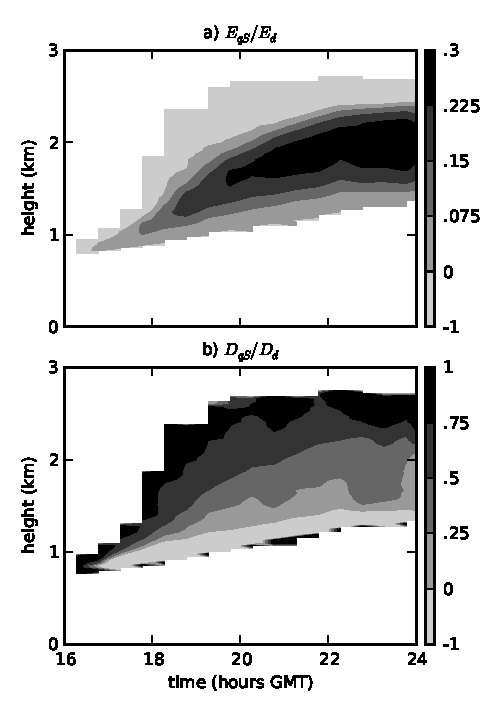
\includegraphics[width=19pc]{./figures/entrainment_ratio_variability}\\
  \caption{Ratio of the total specific water tracer budget a) 
  entrainment and b) detrainment values to the directly calculated 
  values over the duration of the ARM model run.}
  \label{fig:entrainment_ratio_variability}
\end{figure}

\begin{figure}[t]
  \noindent
  \includegraphics[width=39pc,angle=0]{./figures/shell_correction}\\
  \caption{Result of transforming direct entrainment values into 
  equivalent tracer budget values using mean cloud core shell and edge 
  properties.  a) Mean profiles of the total specific humidity in the 
  cloud core (thick black line), cloud core edge (thin black line), 
  cloud core shell (thin grey line), and cloud core environment (thick 
  grey line).  These $q_t$ values are used to transform directly 
  calculated values of b) entrainment and c) detrainment (grey line) 
  into equivalent tracer budget values (black line).  The tracer budget 
  entrainment and detrainment are shown for comparison (dotted lines).}
  \label{fig:Shell_correction}
\end{figure}

\begin{figure}[t]
  \noindent
  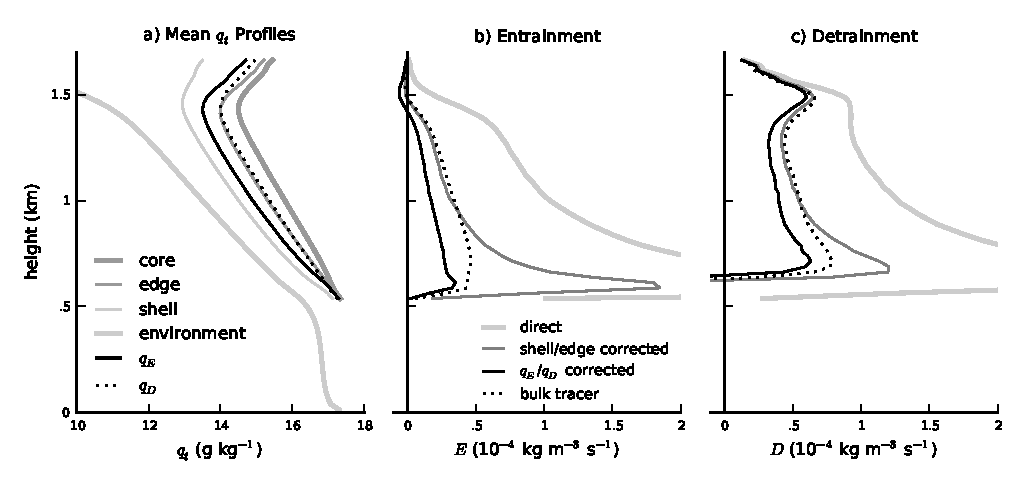
\includegraphics[width=39pc,angle=0]{./figures/reynolds_correction}\\
  \caption{Result of transforming direct entrainment values into 
  equivalent tracer budget values using effective entrainment and 
  detrainment properties.  a) Mean profiles of the effective total 
  specific humidity values being entrained ($q_{entrain}$, black line), 
  and detrained ($q_{detrain}$ dotted line), overlaid on the mean total 
  specific water values of the core, edge, shell and environment.  These 
  $q_t$ values are used to transform directly calculated values of b) 
  entrainment and c) detrainment (grey line) into equivalent tracer 
  budget values (black line).  The Siebesma tracer budget entrainment 
  and detrainment are shown for comparison (dotted lines).}
  \label{fig:Reynolds_correction}
\end{figure}

\begin{figure}[t]
  \noindent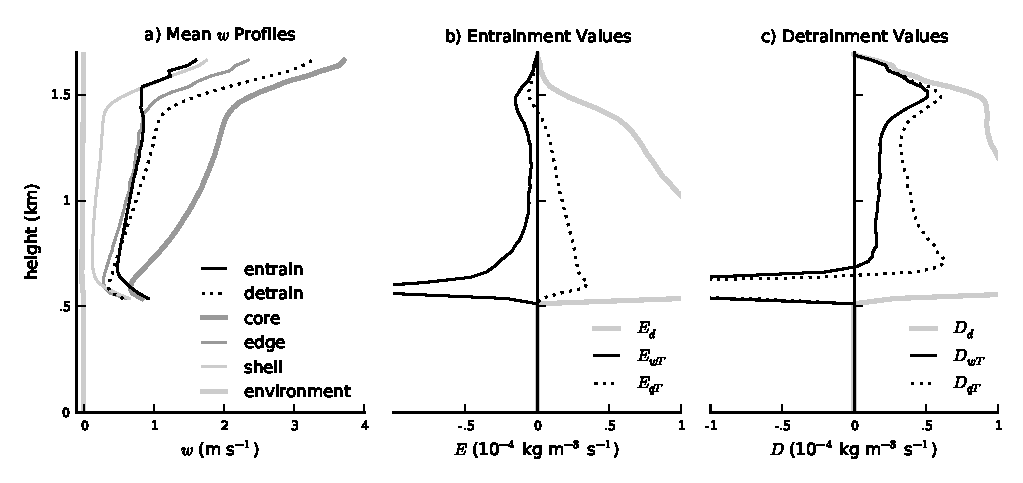
\includegraphics[width=39pc]{./figures/reynolds_correction_w}
  \caption{Result of transforming direct entrainment values into 
  equivalent $w$ budget values.  a) Mean profiles of the effective $w$ 
  values being entrained (black line), and detrained (dotted line), 
  overlaid on the mean $w$ values of the core, edge, shell and 
  environment.  The entrained and detrained $w$ values are used to 
  transform directly calculated values of b) entrainment and c) 
  detrainment (grey line) into equivalent tracer budget values 
  (black line).  The entrainment and detrainment values transformed 
  using $q_t$ are shown for comparison (dotted lines).}
  \label{fig:Reynolds_correction_w}
\end{figure}

\begin{figure}[t]
  \noindent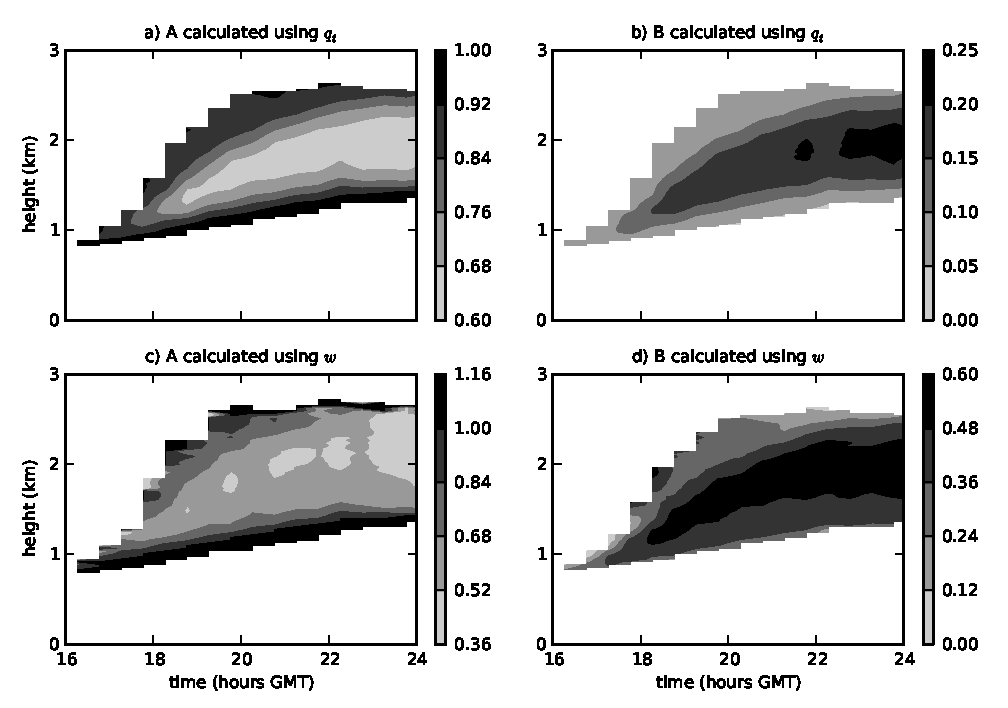
\includegraphics[width=39pc]{./figures/shell_variability}
  \caption{Variation in a) the fraction of core air in a mixture of core 
  and environmental air needed to produce the mean humidity entrained by 
  the clouds, b) the fraction of environmental air in a mixture of core 
  and environmental air needed to produce the mean humidity detrained by 
  the clouds, c) the fraction of core air in a mixture of core and 
  environmental air needed to produce the mean vertical velocity 
  entrained by the clouds, and d) the fraction of environmental air in 
  a mixture of core and environmental air needed to produce the mean 
  vertical velocity detrained by the clouds, over the duration of the 
  ARM model run.
  }
  \label{fig:shell_variability}
\end{figure}

\begin{figure}[t]
  \noindent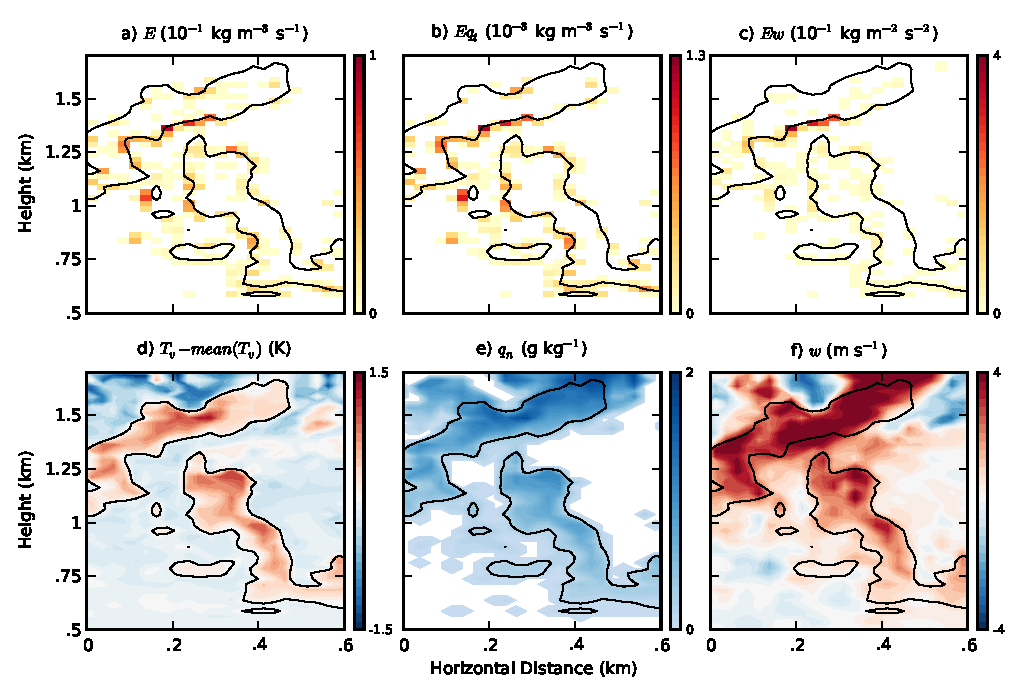
\includegraphics[width=39pc]{./figures/w_entrainment_example}
  \caption{Instantaneous vertical cross-section of directly calculated 
  cloud core mass entrainment (a), humidity entrainment (b), vertical 
  velocity entrainment (c), buoyancy (d), condensed liquid water (e), 
  and vertical velocity (f) of a single model cloud, illustrating the 
  tendency to entrain shell air that is rising faster than the mean 
  shell.  Black lines indicate the edge of the cloud core in each 
  figure.}
  \label{fig:w_entrainment_example}
\end{figure}

\end{document}
